\section{Overview}
\label{sec:analyze_overview}

The 'Analyze Data Source' task examines chosen Data Source(s) using the calculated Reference Trajectory (RefTraj) as ground truth. It is separate funcionality from the requirement-based evaluation (see \nameref{sec:eval}) and is meant to characterize a sensor's behavior in the recorded environment rather than to assess its compliance with a standard. \\\\

The feature can be started using the main menu Process $\rightarrow$ Analyze $\rightarrow$ MLAT \\

Inspectors come in two tiers:

\begin{itemize}
\item Free: always available with any installation
\item \textbf{[Pro]}: require a Professional license
\end{itemize}
\ \\

\begin{figure}[H]
  \centering
  \hspace*{-1.0cm}
    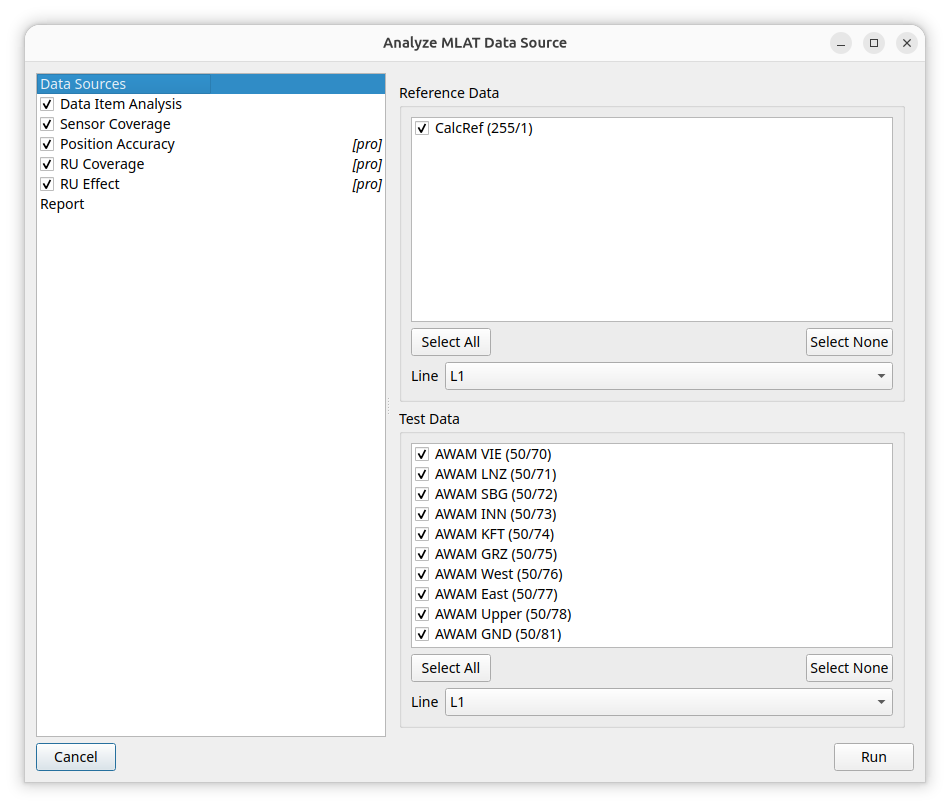
\includegraphics[width=17cm]{figures/analyze_mlat.png}
  \caption{Analyze MLAT dialog}
\end{figure}
